%<dscrpt>Théorème de Pick.</dscrpt>
On se place dans un plan orienté muni d'un repère $( O,(\overrightarrow i, \overrightarrow j))$ orthonormé direct. Les fonctions coordonnées relatives à ce repère sont notées $(x,y)$. Les coordonnées d'un point $M$ du plan sont donc $(x(M),y(M))$.\\
Dans tout le problème, tous les triangles considérés sont non aplatis et, si des coordonnées sont utilisées, il s'agit de coordonnées dans $( O,(\overrightarrow i, \overrightarrow j)) $ sauf si un autre repère est explicitement précisé.\\
Des polygones \emph{fermés sans point double} sont considérés. Un tel polygone est une suite de points $(A_1,A_2,\cdots,A_p)$ tels que
\begin{displaymath}
  A_p = A_1, \hspace{0.5cm} \forall(i,j)\in \llbracket 1,p-1\rrbracket,\; i\neq j \Rightarrow A_i \neq A_j
\end{displaymath}
Les points $A_i$ sont appelés les \emph{sommets} du polygone.\newline
On admet qu'un tel polygone définit deux parties du plan : une \emph{surface polygonale} et une \emph{ligne polygonale} (voir figure \ref{fig:Epick_1}). Il conviendra de les distinguer soigneusement.
\begin{figure}[!ht]
 \centering
 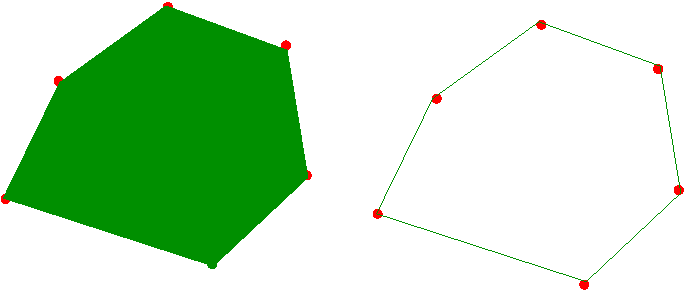
\includegraphics{./Epick_1.pdf}
 \caption{Surface polygonale et ligne polygonale}
 \label{fig:Epick_1}
\end{figure}
On dira en particulier qu'un point $P$ est \emph{strictement à l'intérieur} du polygone si et seulement si il appartient à la surface polygonale sans appartenir à la ligne polygonale.

L'objet de ce problème est le \emph{Théorème de Pick} (1859-1942) qui permet de calculer l'aire de certaines surfaces polygonales en comptant les points à coordonnées entières qu'elles contiennent.

On pourra utiliser librement la propriété fondamentale \emph{d'additivité de l'aire}. L'aire de l'union de deux surfaces polygonales dont l'intersection se réduit à une ligne polygonale est la somme des aires.

\subsection*{I. Systèmes de Cramer}
Pour toute base $(\overrightarrow{u},\overrightarrow{v})$ du plan, notons $\det_{(\overrightarrow{u},\overrightarrow{v})}$ le déterminant dans cette base (forme bilinéaire antisymétrique), notons aussi
\begin{displaymath}
  \Z\overrightarrow{u} + \Z\overrightarrow{v} = \left\lbrace x\overrightarrow{u} + y\overrightarrow{v}, (x,y)\in \Z^2\right\rbrace 
\end{displaymath}
En particulier $\Z\overrightarrow{i} + \Z\overrightarrow{j}$ est l'ensemble des vecteurs à coordonnées entières.
\begin{enumerate}
 \item Question de cours. Montrer que
 \begin{displaymath}
   \det_{(\overrightarrow{u},\overrightarrow{v})}(\overrightarrow{i},\overrightarrow{j})
   \det_{(\overrightarrow{i},\overrightarrow{j})}(\overrightarrow{u},\overrightarrow{v}) = 1
 \end{displaymath}
 Exprimer les coordonnées d'un vecteur $\overrightarrow{w}$ dans la base $(\overrightarrow{u},\overrightarrow{v})$ à l'aide de déterminants dans la base $(\overrightarrow{i},\overrightarrow{j})$.
 \item Soit $(\overrightarrow{u},\overrightarrow{v})$ une base formée de vecteurs de $\Z\overrightarrow{i} + \Z\overrightarrow{j}$. Montrer que 
 \begin{displaymath}
   \Z\overrightarrow{i} + \Z\overrightarrow{j} = \Z\overrightarrow{u} + \Z\overrightarrow{v}
   \Leftrightarrow \det_{(\overrightarrow{i},\overrightarrow{j})}(\overrightarrow{u},\overrightarrow{v})\in\left\lbrace -1, +1\right\rbrace 
 \end{displaymath}

\end{enumerate}

\subsection*{II. Triangles élémentaires}
Un triangle est dit \emph{entier} si et seulement si ses sommets sont à coordonnées entières. Un triangle entier est dit \emph{élémentaire} si et seulement  si les \emph{seuls} points à coordonnées entières qu'il contient sont ses sommets.

Soit $A$, $B$, $C$ un triangle entier tel que $(A,(\overrightarrow{AB},\overrightarrow{AC}))$ est un repère direct (qui n'est pas orthonormé en général).  On note $(X,Y)$ les fonctions coordonnées relatives à ce repère. On désigne par $S$ l'aire de la surface polygonale définie par ce triangle.

\begin{enumerate}
 \item Exprimer $S$ en fonction de $\det(\overrightarrow{AB}, \overrightarrow{AC})$. En déduire que l'aire d'un triangle entier est un multiple de $\frac{1}{2}$.
 
 \item Soit $D$ défini par $D = A + \overrightarrow{AB} + \overrightarrow{AD}$ de sorte que $(A,B,D,C)$ soit un parallélogramme entier.\newline
Soit $P$ un point quelconque du plan. Traduire par des systèmes d'inégalités portant sur $X(P)$, $Y(P)$, $X(P)+Y(P)-1$ le fait que $P$ soit dans la surface polygonale attachée au parallélogramme $(A,B,D,C)$ ou au triangle $(A,B,C)$. 

 \item Montrer que $S=\frac{1}{2}$ entraine $(A,B,C)$ élémentaire.
 
 \item  
 \begin{enumerate}
   \item On suppose qu'il existe un point $Q$ entier tel que $X(Q)\notin \Z$ ou $Y(Q)\notin \Z$. Montrer qu'il existe un point entier $P$ tel que 
   \begin{displaymath}
     0\leq X(P) < 1, \hspace{0.5cm} 0\leq Y(P) < 1 , \hspace{0.5cm} X(P)Y(P) = 0
   \end{displaymath}
   Montrer que le point $P'$ défini par $X(P') = 1 - X(P)$, $Y(P') = 1-Y(P)$ est entier.
   
   \item Montrer que $(A, B, C)$ élémentaire entraine $S = \frac{1}{2}$.
 \end{enumerate}
  
\end{enumerate}

\subsection*{III. Aire et comptages}
Un point est dit entier lorsque ses coordonnées sont entières. Soit $\mathcal P$ un polygone fermé. Il est dit entier lorsque tous les sommets de sa ligne polygonale sont à coordonnées entières. Tous les polygones considérés dans cette partie sont entiers. On note
\begin{itemize}
 \item $a(\mathcal{P})$ : l'aire de la surface polygonale associée.
 \item $i(\mathcal{P})$ : le nombre de points entiers strictement à l'intérieur de $\mathcal P$.
 \item $l(\mathcal{P})$ : le nombre de points entiers sur la ligne polygonale de $\mathcal P$.
\end{itemize}
On dira qu'un polygone fermé est \emph{de Pick} si et seulement si il vérifie
\begin{displaymath}
 a(\mathcal{P}) = i(\mathcal{P}) +\frac{1}{2}l(\mathcal{P}) -1
\end{displaymath}
\begin{enumerate}
 \item Montrer qu'un triangle élémentaire est de Pick.
 \item Soit $\mathcal{P}_1$ et $\mathcal{P}_2$ deux polygones de Pick tels que l'intersection des surfaces associées soit une ligne polygonale (figure \ref{fig:Epick_2}).
\begin{figure}[!ht]
 \centering
 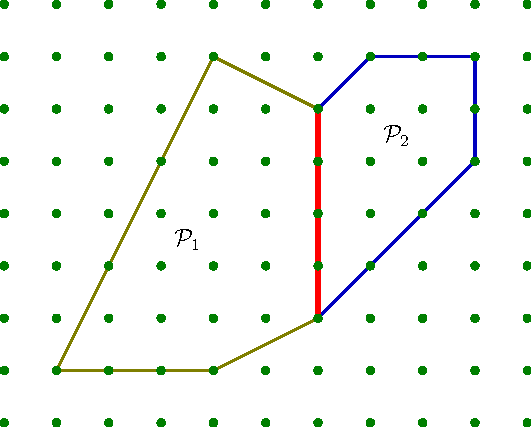
\includegraphics[width=7cm]{./Epick_2.pdf}
 \caption{Union de deux surfaces polygonales entières.}
 \label{fig:Epick_2}
\end{figure}
 Montrer que le polygone associé à $\mathcal{P}_1 \cup \mathcal{P}_2$ est encore de Pick.
 \item Montrer que tout triangle entier est de Pick.
 \item Calculer l'aire de la surface polygonale de la figure \ref{fig:Epick_3}. L'argumentation doit reposer sur un dessin accompagné d'explications soigneusement rédigées.
\begin{figure}[!ht]
 \centering
 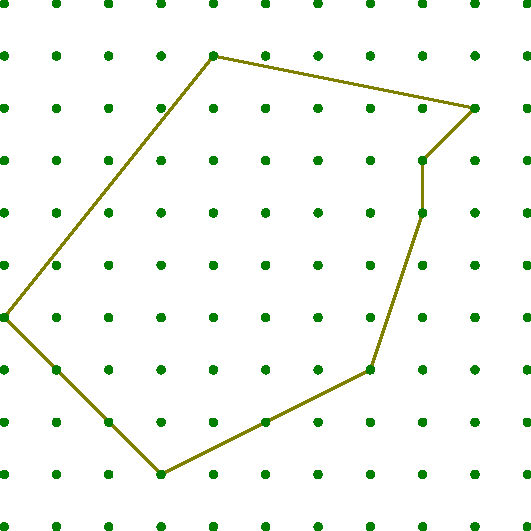
\includegraphics[width=7cm]{./Epick_3.pdf}
 \caption{Une surface polygonale de Pick.}
 \label{fig:Epick_3}
\end{figure}
\end{enumerate}
